% Chapter 4

\chapter{Methodology} % Main chapter title

\label{Chapter4} % For referencing the chapter elsewhere, use \ref{Chapter1} 

\lhead{Chapter 4. \emph{Drawings}} % This is for the header on each page - perhaps a shortened title

%----------------------------------------------------------------------------------------
\section{Overview}
The Dynamic Energy Map is created with a conceptual urban environment
with the following properties:
\begin{enumerate}[i.]
\item Building density and land use pattern are realistic.  
  
  To achieve this, the project used a redevelopment project at Lower
  Hill District, Pittsburgh, PA~\cite{Ramesh2013} as a prototype and
  is created based on extracted topological patterns from this
  redevelopment projec.

\item The number of buildings in the model represents a typical sized
  community that can be served by a district energy
  system~\cite{IDEA2012}.
  
  To achieve this, the original model created under crateria i. is
  duplicated and thus there are 68 buildings in total, within the
  range of a typical district energy system service capacity of 50 to
  150~\cite{IDEA2012}.

\end{enumerate}

The inputs to the dynamic energy map are the energy consumption data
and the urban environment layout. For the conceptual setting, the
energy data is retrieved from the simulation of DOE Benchmark
buildings of new construction which comply with ASHRAE 90.1-2004
Standard~\cite{DOE2015}.

The output of the dynamic energy map is a sequence of 2D or 3D energy
choropleth maps images.

An interface is designed to provide an interactive inspection of the
map sequence and create dynamic data plots (~\fref{fig:flow}). By
replacing the simulated energy data with actual metered energy
consumption data and the conceptual layout with a real urban
environment layout, the same method can be directly applied to the
analysis of a real project.

\begin{figure}[h!]
  \centering
  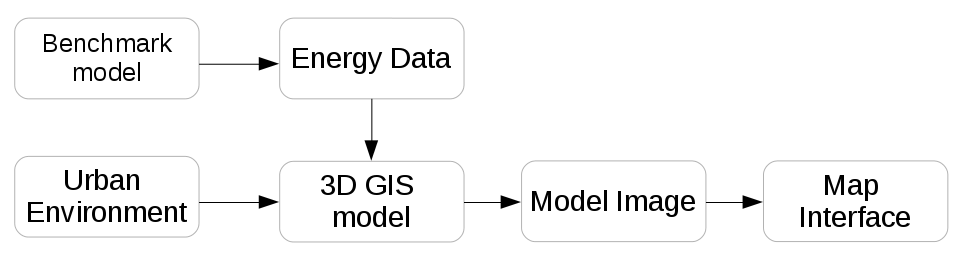
\includegraphics[width=0.7\linewidth]{flow.png}
  \caption[General Work Flow]{General Work Flow}
  \label{fig:flow}
\end{figure}

The major functions of the current dynamic energy map interface
include:
\begin{enumerate}[i.]
\item Comparing heating and cooling demand to identify energy recovery
  opportunities
\item Comparing heating and electricity demand to size co-generation
  system
\end{enumerate}

Details in input output data and the interface design process will be
explained in more details in the following sections.
\newpage
\section{Input}
\subsection{Benchmark Models and Energy Data}
In the Lower Hill District project, the DOE benchmark buildings were
substituted for buildings in the community model in the district
system feasibility analysis. This approach allows for a fast initial
assessment of the district system~\cite{baird2014}.

Following the same approach, the energy profile used in the current
study is retrieved from simulation results of commercial building
benchmark buildings developed by U.S. Department of Energy
(DOE)~\cite{DOE2015}. There are 16 building types in the benchmark
models (\fref{tab:doeModel}). The building types involved in the
current project include: Large Office (LO), Medium Office (MO), Small
Office (SO), Stand-alone Retail (SR), Supermarket (SU), Quick Service
Restaurant (QR), Full Service Restaurant (FR), Large Hotel (LH) and
Midrise Apartment (MA). The two-letter shorthand in the parenthesis
after each building type is used in the building label for the dynamic
map display. The general information for the benchmark buildings are
shown in \tref{tab:doeModel}:

\begin{table}[h!]
  \centering
  \begin{tabular}{l|l|c|c}
    \hline
Building Type Name&Shorthand&  Floor Area (ft2)    & Number of Floors\\
    \hline
Large Office	         &LO&  498,588	      & 12\\
Medium Office	         &MO&  53,628	      & 3\\
Small Office	         &SO&  5,500	      & 1\\
Warehouse	         &WH&  52,045	      & 1\\
Stand-alone Retail       &SR&  24,962	      & 1\\
Strip Mall	         &SM&  22,500	      & 1\\
Primary School	         &PS&  73,960	      & 1\\
Secondary School         &SS&  210,887	      & 2\\
Supermarket	         &SU&  45,000	      & 1\\
Quick Service Restaurant &QR&  2,500          & 1\\
Full Service Restaurant  &FR&  5,500          & 1\\
Hospital	         &HO&  241,351	      & 5\\
Outpatient Health Care   &OP&  40,946	      & 3\\
Small Hotel	         &SH&  43,200	      & 4\\
Large Hotel	         &LH&  122,120	      & 6\\
Midrise Apartment        &MA&  33,740	      & 4\\
    \hline
\end{tabular}
\caption{DOE Benchmark Building General Information~\cite{DOE2015}}
\label{tab:doeModel}
\end{table}

The benchmark buildings comply with the ASHRAE Standard 90.1-2004. The
HVAC system types are shown in \tref{tab:hvac}. The major heating
systems of the benchmark buildings are furnace and boilers, except
that the small hotel and the warehouse has individual space heaters
other than furnaces. The cooling systems are chillers for Large Hotel
(air-based) and Large Office (water-based) and PACU (packed
air-conditioning unit) for other building types.~

\begin{table}[h!]
\centering
\scriptsize
\caption{Benchmark Building HVAC System}
\label{tab:hvac}
%\begin{tabular}{l|p{3cm}|p{4cm}|p{4cm}}
\begin{longtable}{p{2cm}|p{2cm}|p{4cm}|p{4cm}}
  \hline
  & Heating                                & Cooling                                                                     & Air                                                     \\
  \hline
  \hline
  Small Office             & Furnace                                & PACU (packed air-conditioning unit)                                         & SZ CAV (single-zone constant air volume)                \\
  \hline
  Medium Office            & Furnace                                & PACU (packed air-conditioning unit)                                         & MZ VAV (multizone variable air volume)                  \\
  \hline
  Large Office             & Boiler                                 & Chiller (2) water cooled                                                    & MZ VAV (multizone variable air volume)                  \\
  \hline
  Primary School           & Boiler                                 & PACU (packed air-conditioning unit)                                         & CAV (constant air volume)                               \\
  \hline
  Secondary School         & Boiler                                 & Chiller (2) air cooled                                                      & MZ VAV (multizone variable air volume)                  \\
  \hline
  Stand-Alone Retail       & Furnace                                & PACU (packed air-conditioning unit)                                         & SZ CAV (single-zone constant air volume)                \\
  \hline
  Strip Mall               & Furnace                                & PACU (packed air-conditioning unit)                                         & SZ CAV (single-zone constant air volume)                \\
  \hline
  Suprmarket               & Furnace                                & PACU (packed air-conditioning unit)                                         & SZ CAV (single-zone constant air volume)                \\
  \hline
  Quick Service Restaurant & Furnace                                & PACU (packed air-conditioning unit)                                         & CAV (constant air volume)                               \\
  \hline
  Full Service Restaurant  & Furnace                                & PACU (packed air-conditioning unit)                                         & SZ CAV (single-zone constant air volume)                \\
  \hline
  Small Hotel              & ISH (individual space heater), furnace & IRAC (individual room air conditioner), PACU (packed air-conditioning unit) & SZ CAV (single-zone constant air volume)                \\
  \hline
  Large Hotel              & Boiler                                 & Chiller (2) air cooled                                                      & FCU (Fan Coil Unit) and VAV (variable air volume)       \\
  \hline
  Hospital                 & Boiler                                 & Chiller (2) water cooled                                                    & CAV (constant air volume) and VAV (variable air volume) \\
  \hline
  OutPatient Healthcare    & Furnace                                & PACU (packed air-conditioning unit)                                         & CAV (constant air volume) and VAV (variable air volume) \\
  \hline
  Warehouse                & ISH (individual space heater), furnace & PACU (packed air-conditioning unit)                                         & SZ CAV (single-zone constant air volume)                \\
  \hline
  Midrise Apartment        & Furnace                                & PACU-SS                                                                     & SZ CAV (single-zone constant air volume)               \\
  \hline
\end{longtable}
\end{table}

\pagebreak
\subsubsection{Input for Identifing Energy Recovery
  Opportunities}\label{sec:inputRecover}
The major heat rejection sources include heating mode heat rejection
and cooling mode heat rejection. The heat rejection in heating mode
happens during the process of the mixing of conditioned and outside
air. This source of heat rejection is more difficult to capture and is
thus left out from the energy recovery potential calculation in this
study. The current study will only focus on the cooling induced heat
reject. 

The heat rejection in cooling mode happens during the condensing
process when the high temperature refrigerant gas condenses with one
of the following heat rejection forms~\cite{Bhatia2015}:
\begin{itemize}
\item Air cooled unit: ambient air is blown through condensing coils
  and removes heat from the gas refrigerant.
\item Cooling tower: cooled water flow past the condensing unit and
  takes away the heat from the gas refrigerant. The water is then
  cooled through evaporation.
\item Fluid cooler: water is sprayed on the condensing coil with fan
  forced air flowing in the opposite direction. It causes evaporative
  cooling effect that takes away the heat from the gas refrigerant.
\end{itemize}
The ``condenser total heat of rejection''~\cite{Bhatia2015} (THR) in
the condensing process equals to the ``net refrigeration effect''
~\cite{Bhatia2015}(RE, the hourly cooling demand), plus the compressor
input, it can be represented with the following equation:

\begin{equation}\label{eq:reject}
THR = RE * f~\cite{Bhatia2015}
\end{equation}

$f$ is the ``Heat Rejection Factor'' and it is typically between 1.15
and 1.25~\cite{Bhatia2015}. The water-based system has heat rejection
factor closer to 1.15 and the air-based system closer to
1.25~\cite{Bhatia2015}.

To help users identify energy recovery opportunities, the energy
information needed to retrieve include: space heating energy demand
and space cooling energy demand. The space cooling demand (RE in
\eref{eq:reject}) is an indicator for heat rejection that could be
recovered and shared within a single building or a building group.

From \tref{tab:heatFuel}, Large Hotel, Medium Office, Midrise
Apartment, OutPatient Healthcare, Small Hotel and Stand-alone Retail
use both electricity and natural gas for space heating, the rest of
the building types uses only natural gas for space heating. We thus
use the EnergyPlus simulation output parameters
``heating:electricity'' and ``heating:gas'' to represent the space
heating demand of reference buildings.
\begin{table}[h]
\centering
\caption{Annual Total Heating Demand by Fuel Type~\cite{DOE2015}}
\label{tab:heatFuel}
\begin{tabular}{lll}
  \hline
                       & Electricity {[}kBtu{]} & Gas {[}kBtu{]} \\
  \hline
  \hline
FullServiceRestaurant  & 0.0                    & 856637.1       \\
Hospital               & 0.0                    & 14045664.0     \\
LargeHotel             & 843.6                  & 2960506.8      \\
LargeOffice            & 0.0                    & 4741180.3      \\
MediumOffice           & 450791.3               & 192226.8       \\
MidriseApartment       & 56.9                   & 494959.6       \\
OutPatient             & 199581.9               & 2881638.9      \\
PrimarySchool          & 0.0                    & 1579186.5      \\
QuickServiceRestaurant & 0.0                    & 383297.2       \\
SecondarySchool        & 0.0                    & 7746443.0      \\
SmallHotel             & 52129.9                & 450393.2       \\
SmallOffice            & 0.0                    & 66631.5        \\
Stand-aloneRetail      & 6966.5                 & 976583.4       \\
StripMall              & 0.0                    & 1013188.1      \\
SuperMarket            & 0.0                    & 3043905.2      \\
Warehouse              & 0.0                    & 1039850.2     \\
  \hline
\end{tabular}
\end{table}

\begin{figure}[h!]
  \centering
  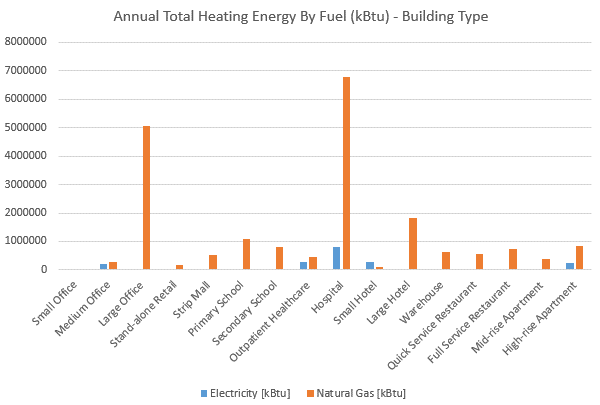
\includegraphics[width=0.7\linewidth]{heatFuel.png}
  \caption[Heating Fuel]{Heating Fuel}
  \label{fig:heatFuel}
\end{figure}
Electricity is the only fuel used for space cooling~\cite{DOE2015},
thus the EnergyPlus output parameter ``cooling:electricity'' is used
to represent space cooling demand. According to the suggested heat
rejection factor~\cite{Bhatia2015}, the heat recovery potential will
be calculated with $f = 1.15$ for Large Office and Hospital, and
$f = 1.25$ for the remaining building types:
\begin{equation}\label{eq:recover}
\text{Heat Recovery Potential} = \text{cooling:electricity} \times f
\end{equation}

In summary, to facilitate identification of energy recovery
opportunities for single buildings and within building groups, the
hourly ``heating:electricity'', ``heating:gas'' and
``cooling:electricity'' output will be extracted from energyPlus
simulation of DOE Commercial benchmark buildings.

\subsubsection{Input for Sizing District Co-generation
  System}
For the sizing of a district co-generation system, the relevant
information needed are the total heating demand, and the total
electricity demand. The general principle used in Lower Hill District
project ~\cite{baird2014} is to use the minimum total heat demand
(space heating and service hot water) over time to assess the minimum
capacity of electricity generation ($E_{heat}$) such that its heat
bi-product from electricity generation will always be consumed. The
maximum total electricity demand ($E_{elec}$) is used for assessing
the capacity of a backup system or a second phase system development
by $C_{backup} = E_{elec} - E_{heat}$ where $C_{backup}$ is the
capacity of electricity generation for the backup system or
second-phase development.

Heating demand assessed in the sizing of co-generation system is
different from the energy recovery use case in \sref{sec:inputRecover}
. It contains the space heating demand and the service hot water
demand. From the summary files of benchmark models, the fuel used for
providing service hot water is natural gas for all building types
(\tref{tab:hotWater})
\begin{table}[h!]
\centering
\caption{Service Hot Water by Fuel Type}
\label{tab:hotWater}
\begin{tabular}{l|l|l}
  \hline
                       &  Electricity {[}kBtu{]} & Gas {[}kBtu{]} \\
  \hline
  \hline
FullServiceRestaurant  & 0 & 253664.3       \\
Hospital               & 0 & 719402.7       \\
LargeHotel             & 0 & 6793934.2      \\
LargeOffice            & 0 & 231381.1       \\
MediumOffice           & 0 & 34178.3        \\
MidriseApartment       & 0 & 289719.3       \\
OutPatient             & 0 & 44054.5        \\
PrimarySchool          & 0 & 174768.0       \\
QuickServiceRestaurant & 0 & 82071.5        \\
SecondarySchool        & 0 & 441512.2       \\
SmallHotel             & 0 & 394017.1       \\
SmallOffice            & 0 & 10928.3        \\
Stand-aloneRetail      & 0 & 0.0            \\
StripMall              & 0 & 0.0            \\
SuperMarket            & 0 & 23799.7        \\
Warehouse              & 0 & 0.0            \\
  \hline
\end{tabular}
\end{table}

The output parameter ``electricity:facility'' was extracted to
represent the total electricity demand.

\pagebreak
\subsection{3D GIS Model Geometry}
The conceptual community model is constructed in
CityEngine~\cite{cityEngine2015}. CityEngine is a software developed
by Esri~\cite{Esri2015}. It can aggregate geographic information into
buildings and is capable of smoothly transition models to
ArcGIS\cite{ArcGIS2015}, one of the widely applied tools for
Geo-referenced data presentation and analysis. Buildings in CityEngine
is defined with ``rules'' using CGA (Computer Generated Architecture)
shape grammar that is unique to CityEngine. The rule-based modeling of
urban environment enables fast construction and easy adjustability of
urban density, skyline and terrain control. It also enables easy
aggregation of Energy profile data into 3D urban environment models,
which is difficult to do in the current ArcGIS, the technical details
will be explained in \aref{AppendixA}.

Although the urban environment in this study is a conceptual setting,
we still want it to reflect the topological and density pattern in a
real urban environment. To construct the model, we first extracted the
topological pattern from an existing urban design project, the Mellon
Arena Project~\cite{baird2014} (\fref{fig:mellonArena}.  There are
eight building types in the project: Residential (43\%), Town House
(2.9\%), Community Center (0.4\%), Commercial (3.8\%), Office (19\%),
Hotel (4.7\%), Cinema (1.4\%) and Garage (24.7\%).

\begin{figure}[h!]
  \centering
  \begin{subfigure}{0.5\textwidth}
  \centering
  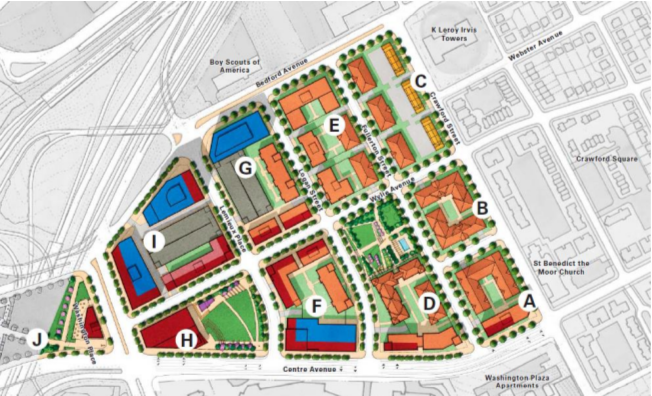
\includegraphics[width=\linewidth]{mellonArena}
  \caption[Mellon Arena Site Plan]{Mellon Arena Project Site Plan View}
  \label{fig:mellonArena}
\end{subfigure}
~
\begin{subfigure}{0.3\textwidth}
  \centering
  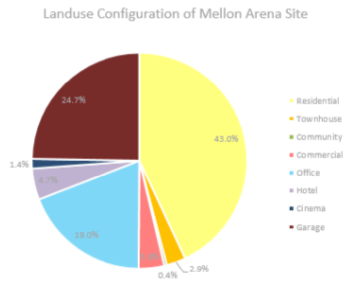
\includegraphics[width=\linewidth]{mellonPie}
  \caption[Mellon Arena Site Land Use]{Mellon Arena Site Land use Configuration}
  \label{fig:mellonPie}
\end{subfigure}
\end{figure}
The 16 building types in DOE commercial benchmark models do not
perfectly correspond to those in the Mellon Arena Site. In order to
adapt the topological pattern of the Mellon Arena Project, a mapping
(function) from building types of Mellon Arena Site to building types
of DOE models is created as is shown in \tref{tab:typeMap}.
\begin{table}[h!]
  \centering
  \begin{tabular}{c| c| c}
    \hline
    Mellon Arena Type &Probability &DOE Building Type\\
    \hline
    \hline
    Hotel &50\%&Large Hotel\\
    \cline{2-3}
    &50\%&Small Hotel\\
    \hline
    Office &30\%&Large Office\\
    \cline{2-3}
    &30\%&Medium Office\\
    \cline{2-3}
    &30\%&Small Office\\
    \hline
    Residential &100\%&Midrise Appartment\\
    \cline{1-2}
    Townhouse &100\%&\\
    \hline
    Commercial &25\%&Full Service Restaurant\\
    \cline{2-3}
    $+$ Cinema $+$&25\%&Quick Service Restaurant\\
    \cline{2-3}
    Community &25\%&Super Market\\
    \cline{2-3}
    Center &25\%&Stand-alone Retail\\
    \hline
  \end{tabular}
  \caption{Mapping of Mellon Arena to Building Types of DOE benchmark model}
  \label{tab:typeMap}
\end{table}

The four major building sectors involved in the current project are
residential, commercial, office and hotel. Their topological pattern
is represented in Figure \ref{fig:mellonTop}. The conceptual model
construction follows the building type topological pattern and the
urban density as the Mellon Arena Project (\fref{fig:sitePlan})

\begin{figure}[h!]
  \centering
  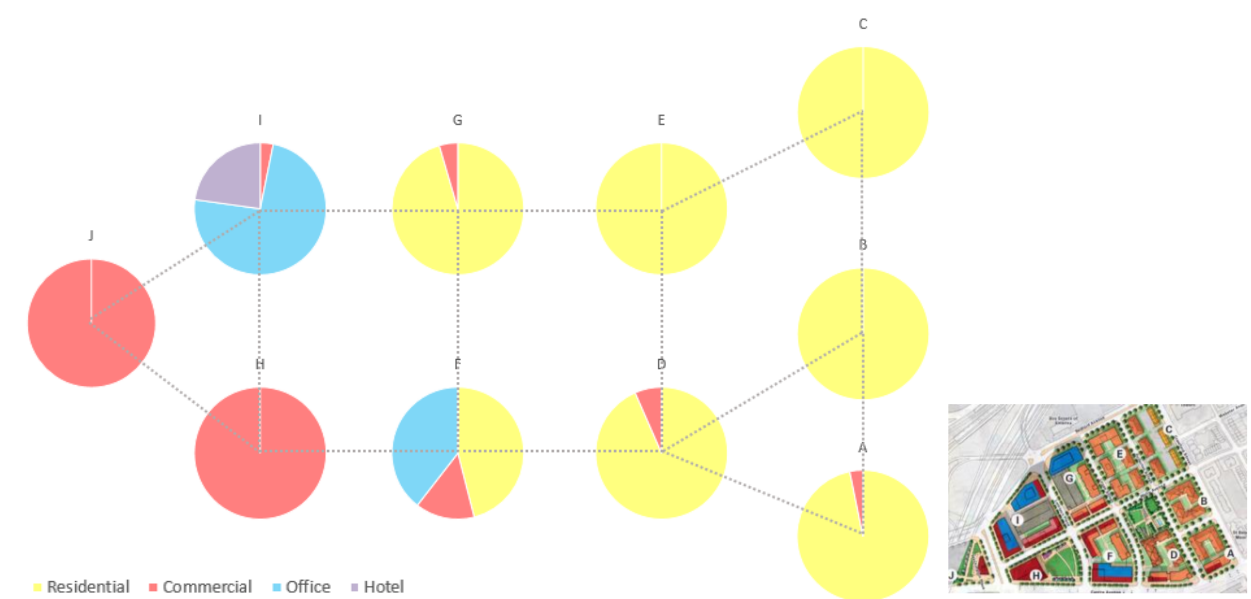
\includegraphics[width=\linewidth]{mellonTop}
  \caption[Building Type Topology]{Building Type Topological Pattern, Mellon Arena}
  \label{fig:mellonTop}
\end{figure}

\begin{figure}[h!]
  \centering
  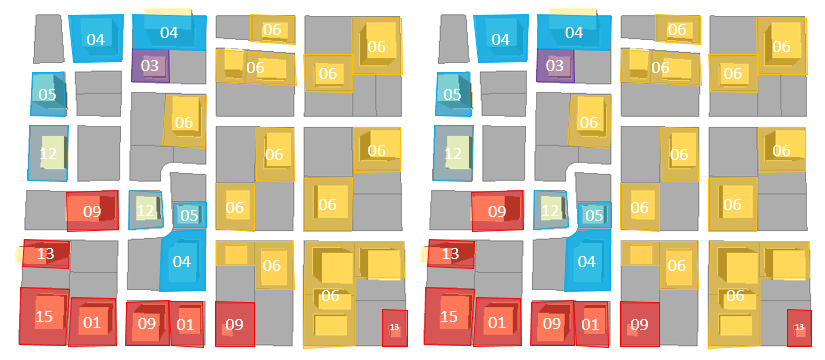
\includegraphics[width=\linewidth]{sitePlan}
  \caption[Conceptual Model Site Plan]{Site Plan of Conceptual Model}~ (01: Full Service
  Restaurant, 03: Large Hotel, 04: Large Office, 05: Medium Office,
  \\06: Midrise Apartment, 09: Quick Service Restaurant, 12: Small
  Office, \\13: Stand-alone Retail, 15: Super Market)
  \label{fig:sitePlan}
\end{figure}